\documentclass[english, 12pt, aspectratio=169]{beamer}
\usepackage{amsmath,amssymb,amsthm,amsfonts}
\usepackage{array}
\usepackage[round]{natbib}
\renewcommand{\bibsection}{}
\usepackage{url}
% \usepackage{fontawesome}
\usepackage{graphicx}
\usepackage{booktabs}
\usepackage{multirow}
\usepackage{doi}
\usepackage[export]{adjustbox} % for framed includegraphics
\usetheme{metropolis}
\usepackage[default]{sourcesanspro}
\usepackage{tcolorbox}
\usepackage{fontawesome} % fontawesome icons
\usepackage{tikz}
\usepackage{svg}
\usepackage{pdfpages}
\usetikzlibrary{positioning, arrows, fadings,decorations.pathmorphing,arrows.meta, shapes.arrows}
\tikzset{
  % Define standard arrow tip
  >=stealth',
  % Define style for boxes
  punkt/.style={
    rectangle,
    rounded corners,
    draw=black, very thick,
    text width=6.5em,
    minimum height=10em,
    minimum width = 10em
    text centered},
  % Define arrow style
  pil/.style={
    ->,
    thick,
    shorten <=2pt,
    shorten >=2pt,}
}

%% colors
\definecolor{nicegreen}{HTML}{008000}
\definecolor{niceblue}{RGB}{30, 126, 229}
\definecolor{nicered}{RGB}{216, 27, 96}
\definecolor{lightlightgray}{RGB}{211,211,211} % for tikz diagram
%\definecolor{lightred}{RGB}{249,174,174} % for tikz diagram
%\definecolor{lightred}{RGB}{255, 204, 118} % for tikz diagram
\definecolor{lightred}{RGB}{253, 169, 104} % for tikz diagram
\definecolor{dark2green}{RGB}{27, 158, 119}
\definecolor{dark2purple}{RGB}{117, 112, 179}
\definecolor{dark2orange}{RGB}{217, 95, 2}
\definecolor{chineseBlue}{RGB}{60, 88, 152}
\definecolor{metallicBlue}{RGB}{41, 72, 125}
\definecolor{wildBlueYonder}{RGB}{156, 178, 206}
\definecolor{gainsboro}{RGB}{212, 216, 232}
\setbeamercolor{frametitle}{bg = metallicBlue}
\setbeamercolor{progress bar}{fg = metallicBlue}
\setbeamercolor{alerted text}{fg=dark2orange}

% red from R ; % blue from R ; % green from R Set 1
\definecolor{Rred}{RGB}{228, 26, 28}
\definecolor{Rgreen}{RGB}{77, 175, 74}
\definecolor{Rblue}{RGB}{55, 126, 184}

\usepackage{hyperref}
\hypersetup{
  pdftitle={Simulation Studies for Methodological Research in Psychology},
  pdfsubject={Björn Siepe}
}



\date{$\star$ Psychological Methods Lab, Department of Psychology, University of Marburg}
\title{~\\ ~ \\ \textbf{Simulation Studies for Methodological Research in Psychology}}
\author{\textbf{Björn S. Siepe}\textsuperscript{$\star$}, František Bartos, Tim P. Morris, Anne-Laure Boulesteix, Daniel Heck, Samuel Pawel}
\institute{
  SIPS 2024. Slides available at \url{htpps://bsiepe.github.io}
}
\titlegraphic{
  \includegraphics[width = 0.2\textwidth]{pics/UMR-logo.png}
}

% TODOS
% slide 9: doesn't need to be as extensive
% template: make example/explanation text more visually distinct
% add qr code
% slide 7: maybe just show upper row first
% slide 5: boxes for parameters, metrics,... could be in a light grey


% Plan:
% 1 slide intro
% 1 slide simulation study importance
% 1 slide review results
% 1 slide ADEMP
% 1 slide (dis-)advantages


\usepackage{Sweave}
\begin{document}
\Sconcordance{concordance:SIPS24-Bjoern-Siepe.tex:SIPS24-Bjoern-Siepe.Rnw:1 98 1 1 0 %
208 1}


\begin{frame}[noframenumbering, plain]
   \titlepage
 \nocite{PawelKookReeve2023}
 \end{frame}


\begin{frame}{Simulation Studies}
        \begin{tcolorbox}[colframe=chineseBlue]
            ``Simulation studies are \alert{\textbf{experiments}} and should be treated as such by authors and editors''(Hauck \& Anderson, 1984)
        \end{tcolorbox}
          % \vspace{-1em}
      \begin{itemize}
      \pause
        \item Most prominent tool for methodological research in psychology
        \pause
        \item Highly influential 
        \pause
      \end{itemize}
      \centering
              
\includegraphics[width=0.7\textwidth,frame]{pics/hubentler.png}
              \nocite{Hauck1984}
          
\end{frame}









\begin{frame}{Literature Review}
\begin{tcolorbox}[colframe=chineseBlue]
            ``\emph{Statisticians ... often pay too little attention to their own principles of design}''(Hoaglin \& Andrews, 1975)
          \end{tcolorbox}
          \vspace{-1em}
  \begin{columns}
    \begin{column}{0.5\textwidth}
      \begin{block}{}
          \centering
          
\includegraphics[width = 0.8\linewidth,frame]{pics/hoaglin.png}
          
\includegraphics[width = 0.8\linewidth,frame]{pics/burton.png}
          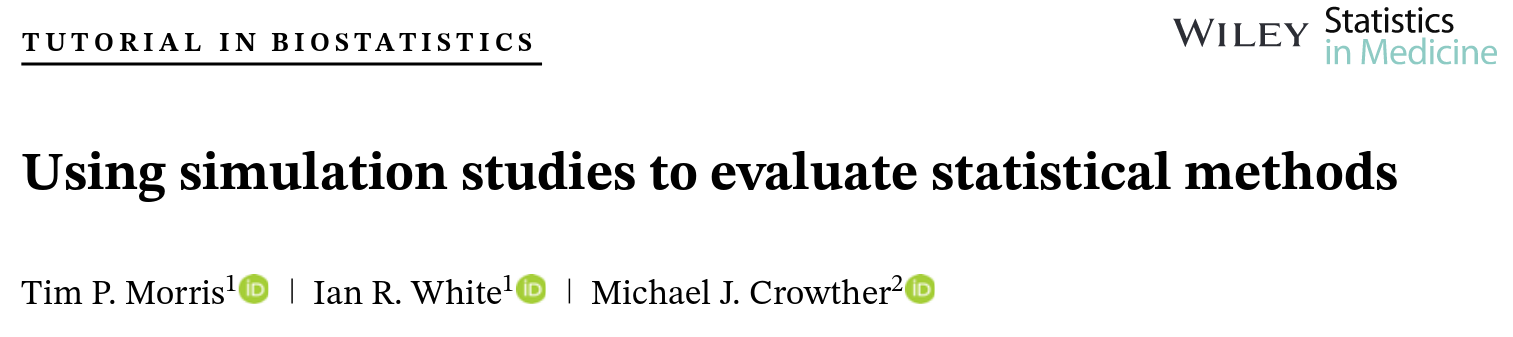
\includegraphics[width = 0.8\linewidth,frame]{pics/morris.png}
          \nocite{Hoaglin1975}
          \pause
      \end{block}
    \end{column}
    \begin{column}{0.5\textwidth}
      \begin{block}{}
      \textbf{This project:}
      \pause
        \begin{itemize}
          \item Review of \alert{100 recent simulation studies} in psychology
          \pause
          \item Majority does not provide code
          \pause
          \item Majority does not provide enough information on the uncertainty of results
        \end{itemize}
      \end{block}
      \end{column}
    \end{columns}
\end{frame}


% \begin{frame}{Main Results}
% \pause
%    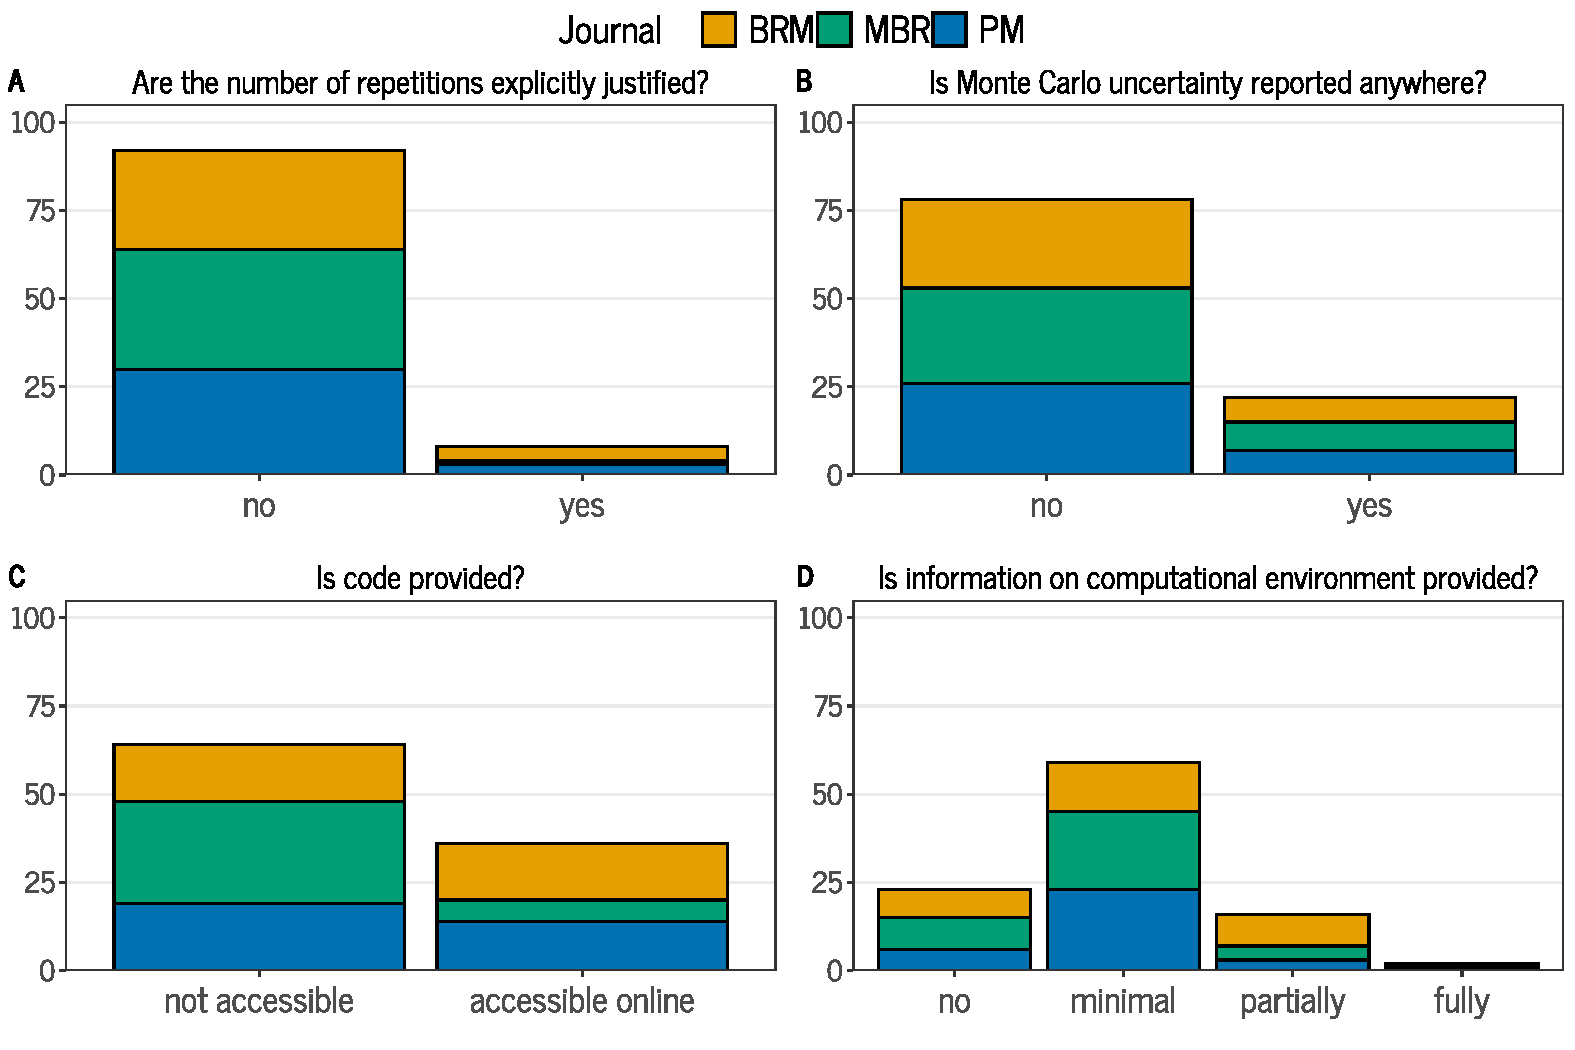
\includegraphics{pics/review-results.pdf}
% \end{frame}




\begin{frame}{Towards improved reporting}
  \begin{block}{}
  \centering
  
\includegraphics[width = 0.6\linewidth,frame]{pics/ademprereg.png}

  \begin{itemize}
  \pause
    \item Protocol template based on \alert{\textbf{ADEMP structure}}
          \citep{Morris2019} + \alert{\textbf{open~science}} +
          \alert{\textbf{reproducibility}} aspects
    % \item Purposes: \alert{preregistration}, \alert{reporting/planning/reviewing
    %       blueprint}
    \pause
    \item \alert{\textbf{Different versions}}: \LaTeX, Overleaf, MS/Libre office, Google
    docs
    \pause
    \item \alert{\textbf{Living
          document}}:          \href{https://github.com/bsiepe/ADEMP-PreReg}{https://github.com/bsiepe/ADEMP-PreReg}
    \end{itemize}
  \end{block}

  \vspace{-1.5em}
  \nocite{Siepe2023}
  \flushleft {\tiny \color{gray}
    \href{https://doi.org/10.1214/ss/1009213726}{ADEMP: doi.org/10.1214/ss/1009213726},
    \href{https://doi.org/10.31234/osf.io/ufgy6}{ADEMP-PreReg: doi.org/10.31234/osf.io/ufgy6}
    }
 % \href{https://www.overleaf.com/latex/templates/ademp-prereg-simulation-study-template/dkhtxjtmpbfj}{overleaf.com/latex/templates/ademp-prereg-simulation-study-template/dkhtxjtmpbfj}}

\end{frame}

% \begin{frame}{The ADEMP-PreReg template}
%   \begin{columns}
%     \begin{column}{0.5\textwidth}
%   \begin{block}{}
%     \begin{enumerate}
%     \item Instructions
%     \item General information
%     \item \alert{\textbf{A}}ims
%     \item \alert{\textbf{D}}ata-generating mechanism
%     \item \alert{\textbf{E}}stimands and targets
%     \item \alert{\textbf{M}}ethods
%     \item \alert{\textbf{P}}erformance Measures
%     \item Computational details
%     \pause
%     \end{enumerate}
%     \nocite{Burton2006}
%   \end{block}
% \end{column}
% \begin{column}{0.5\textwidth}
%   \centering
%   \vspace{1em}
% 
%     % \only<1>{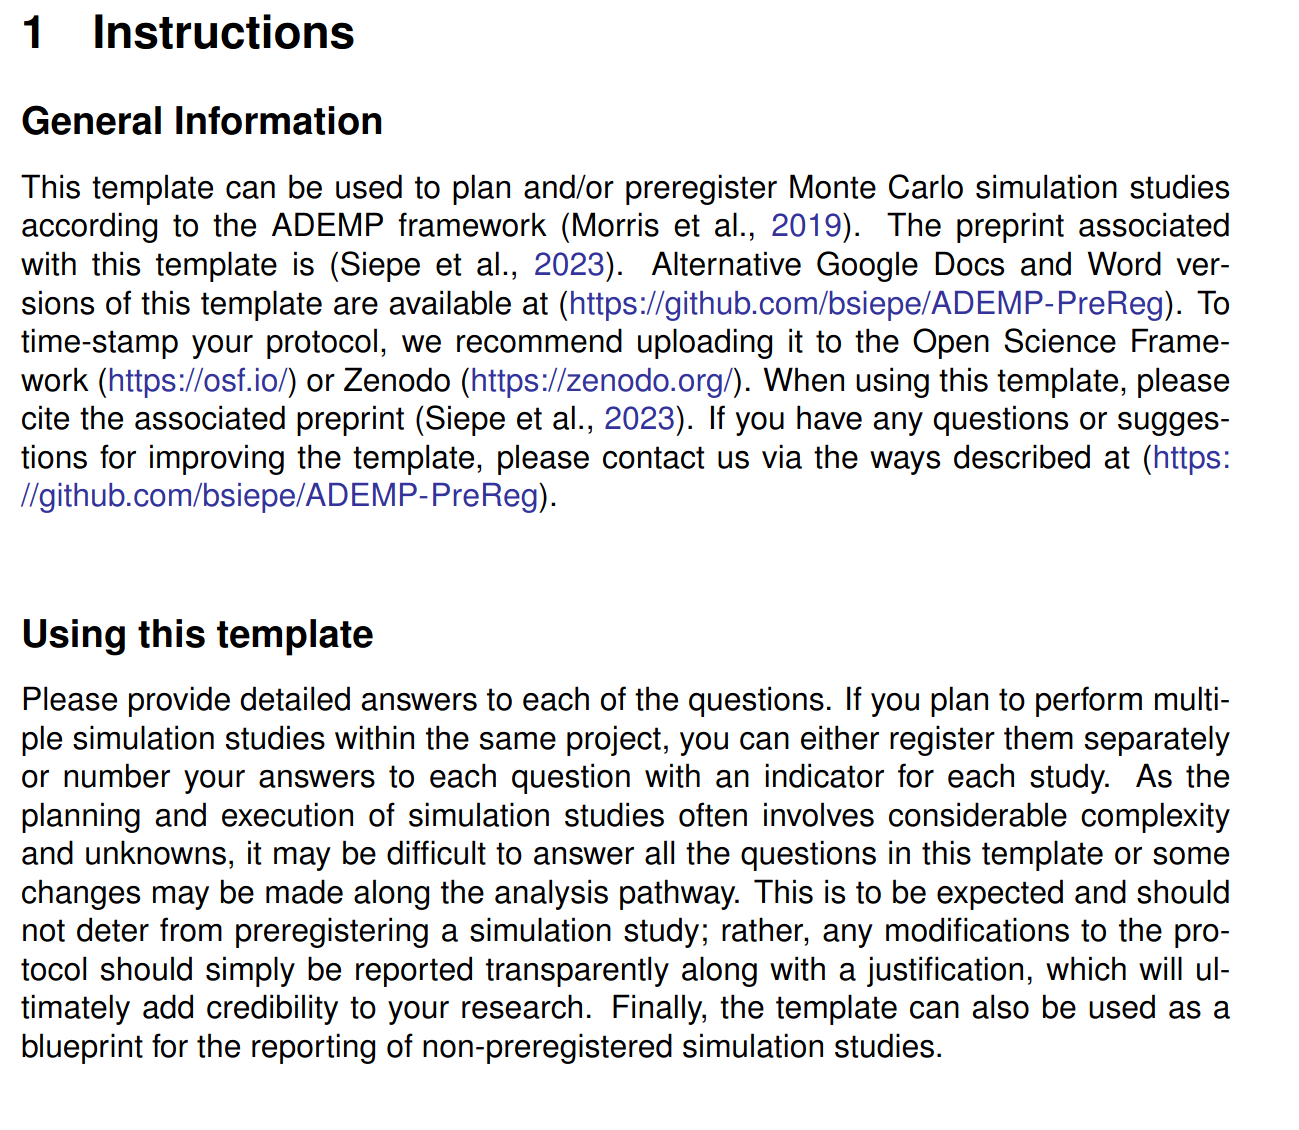
\includegraphics[width=\textwidth,frame]{pics/1instructions.png}}
%     % \only<2>{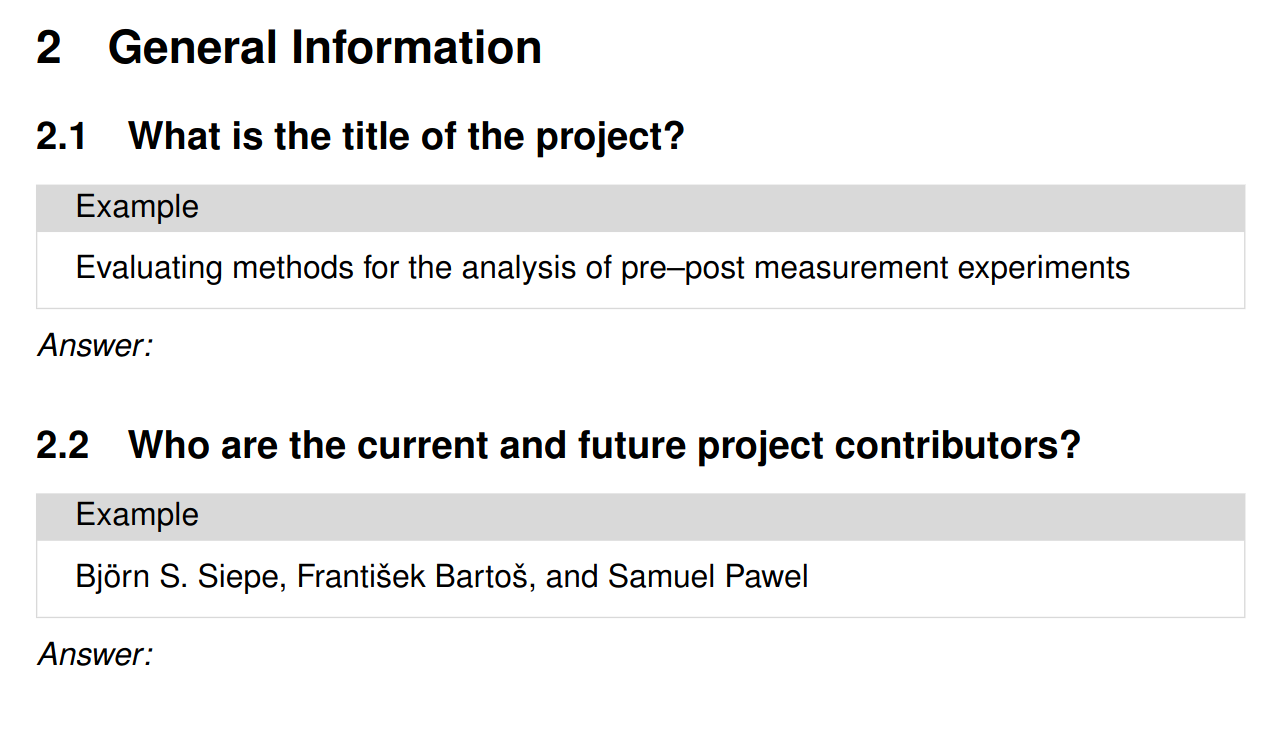
\includegraphics[width=\textwidth,frame]{pics/2general.png}}
%     % \only<3>{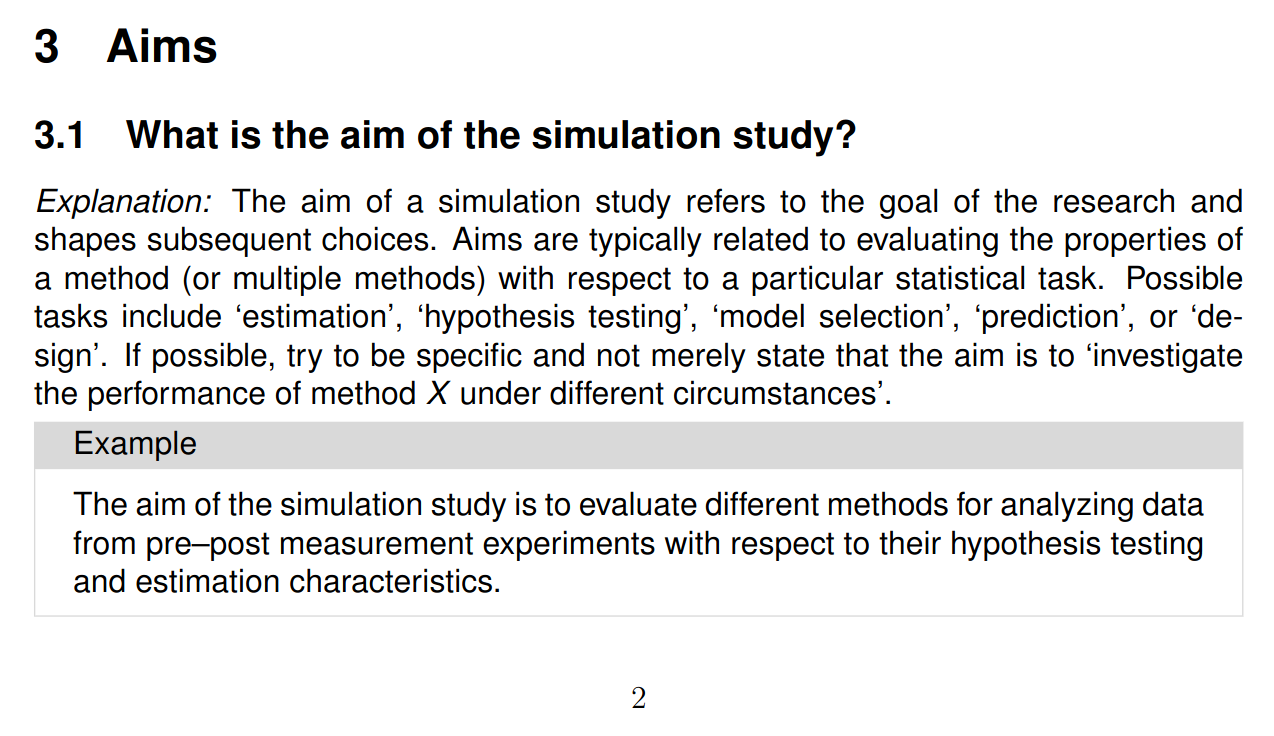
\includegraphics[width=\textwidth,frame]{pics/3aims.png}}
%     % \only<4>{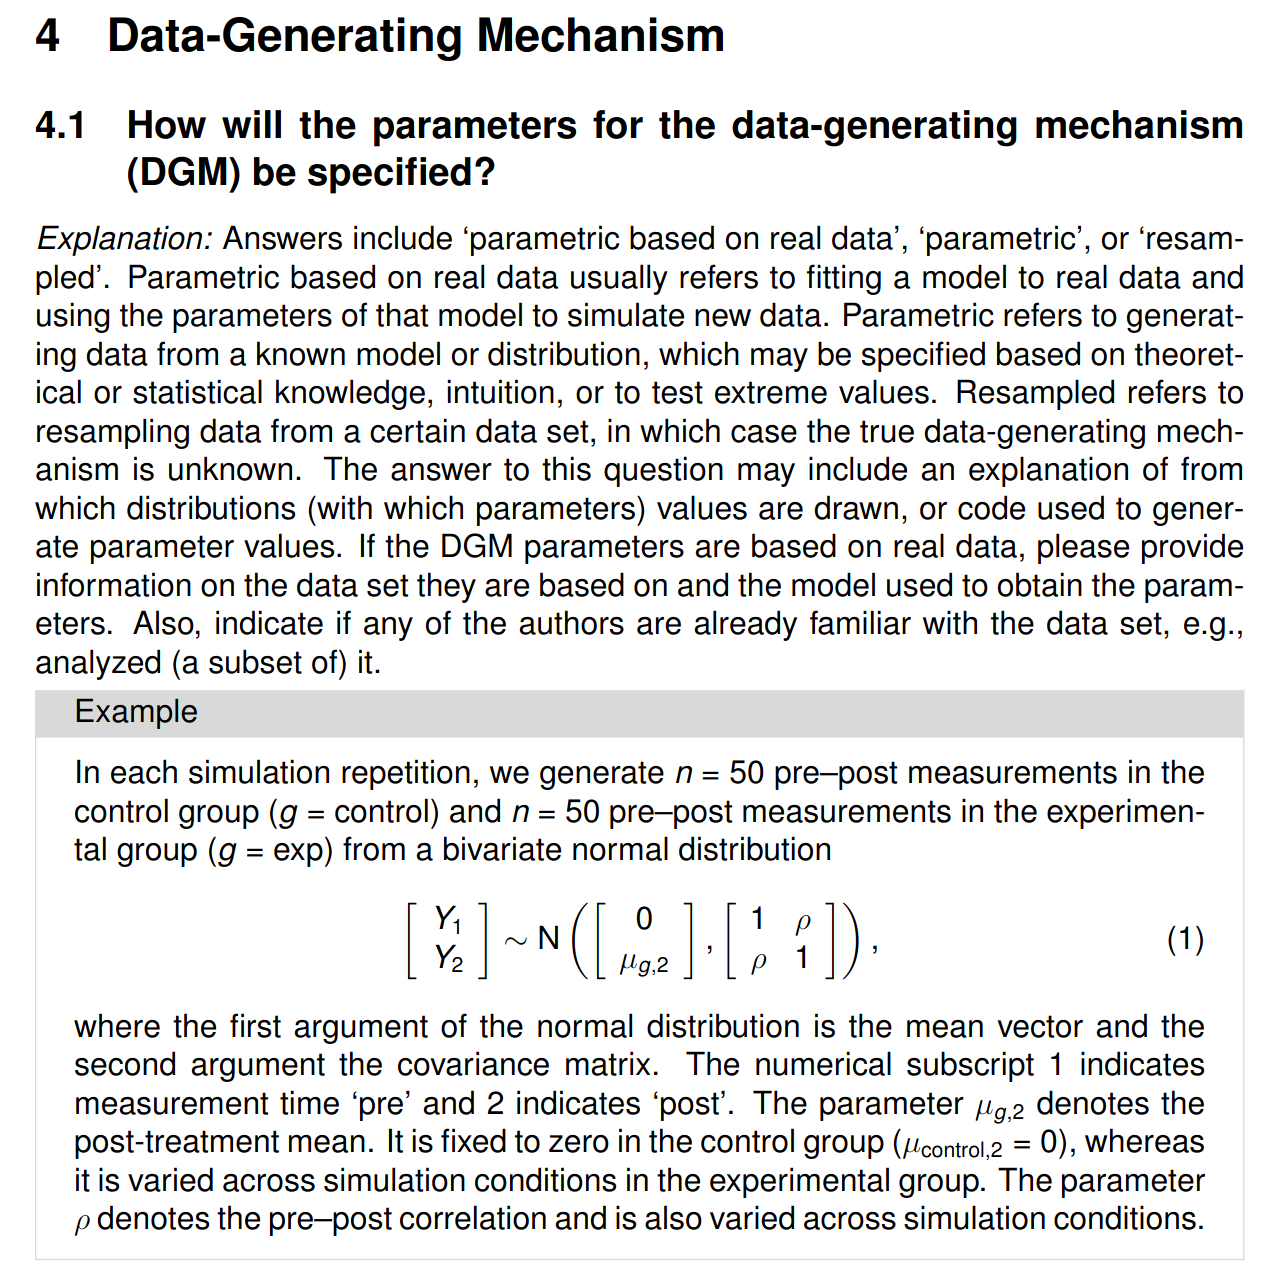
\includegraphics[width=\textwidth,frame]{pics/4dgm.png}}
%     % \only<5>{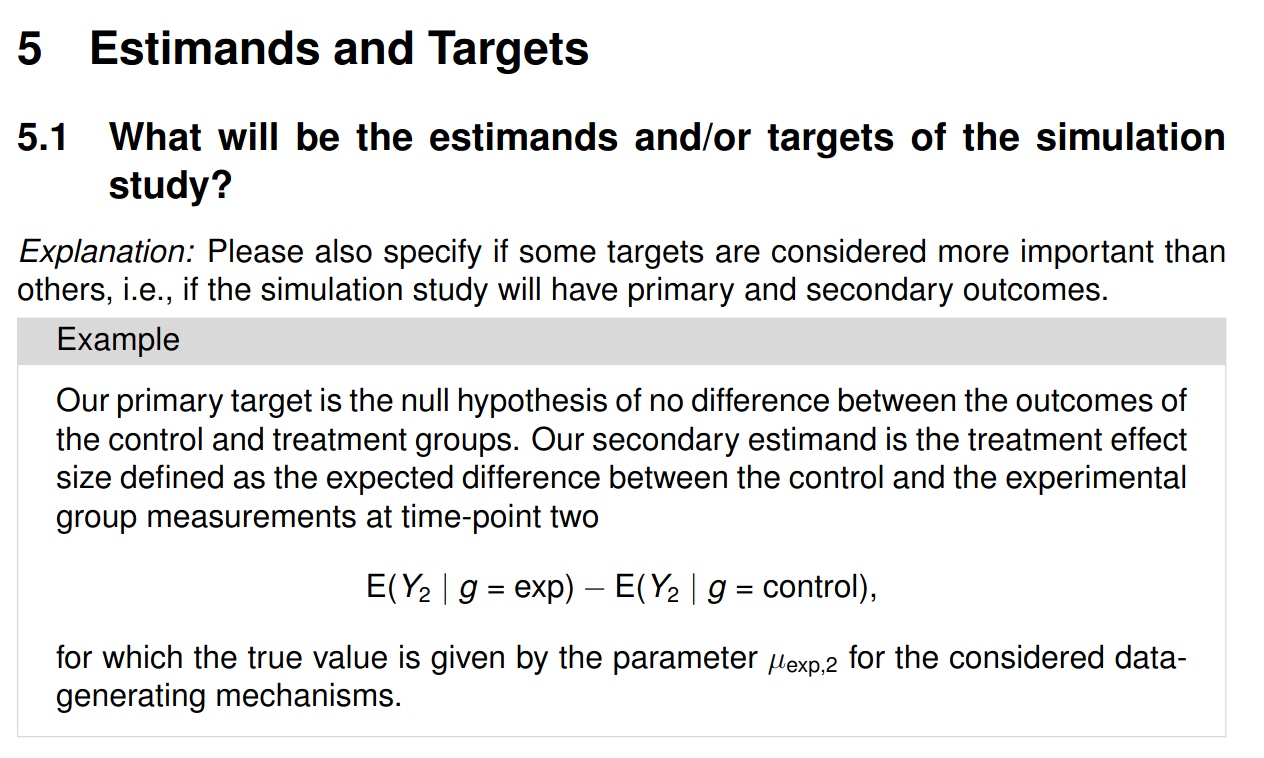
\includegraphics[width=\textwidth,frame]{pics/5estimands.png}}
%     % \only<6>{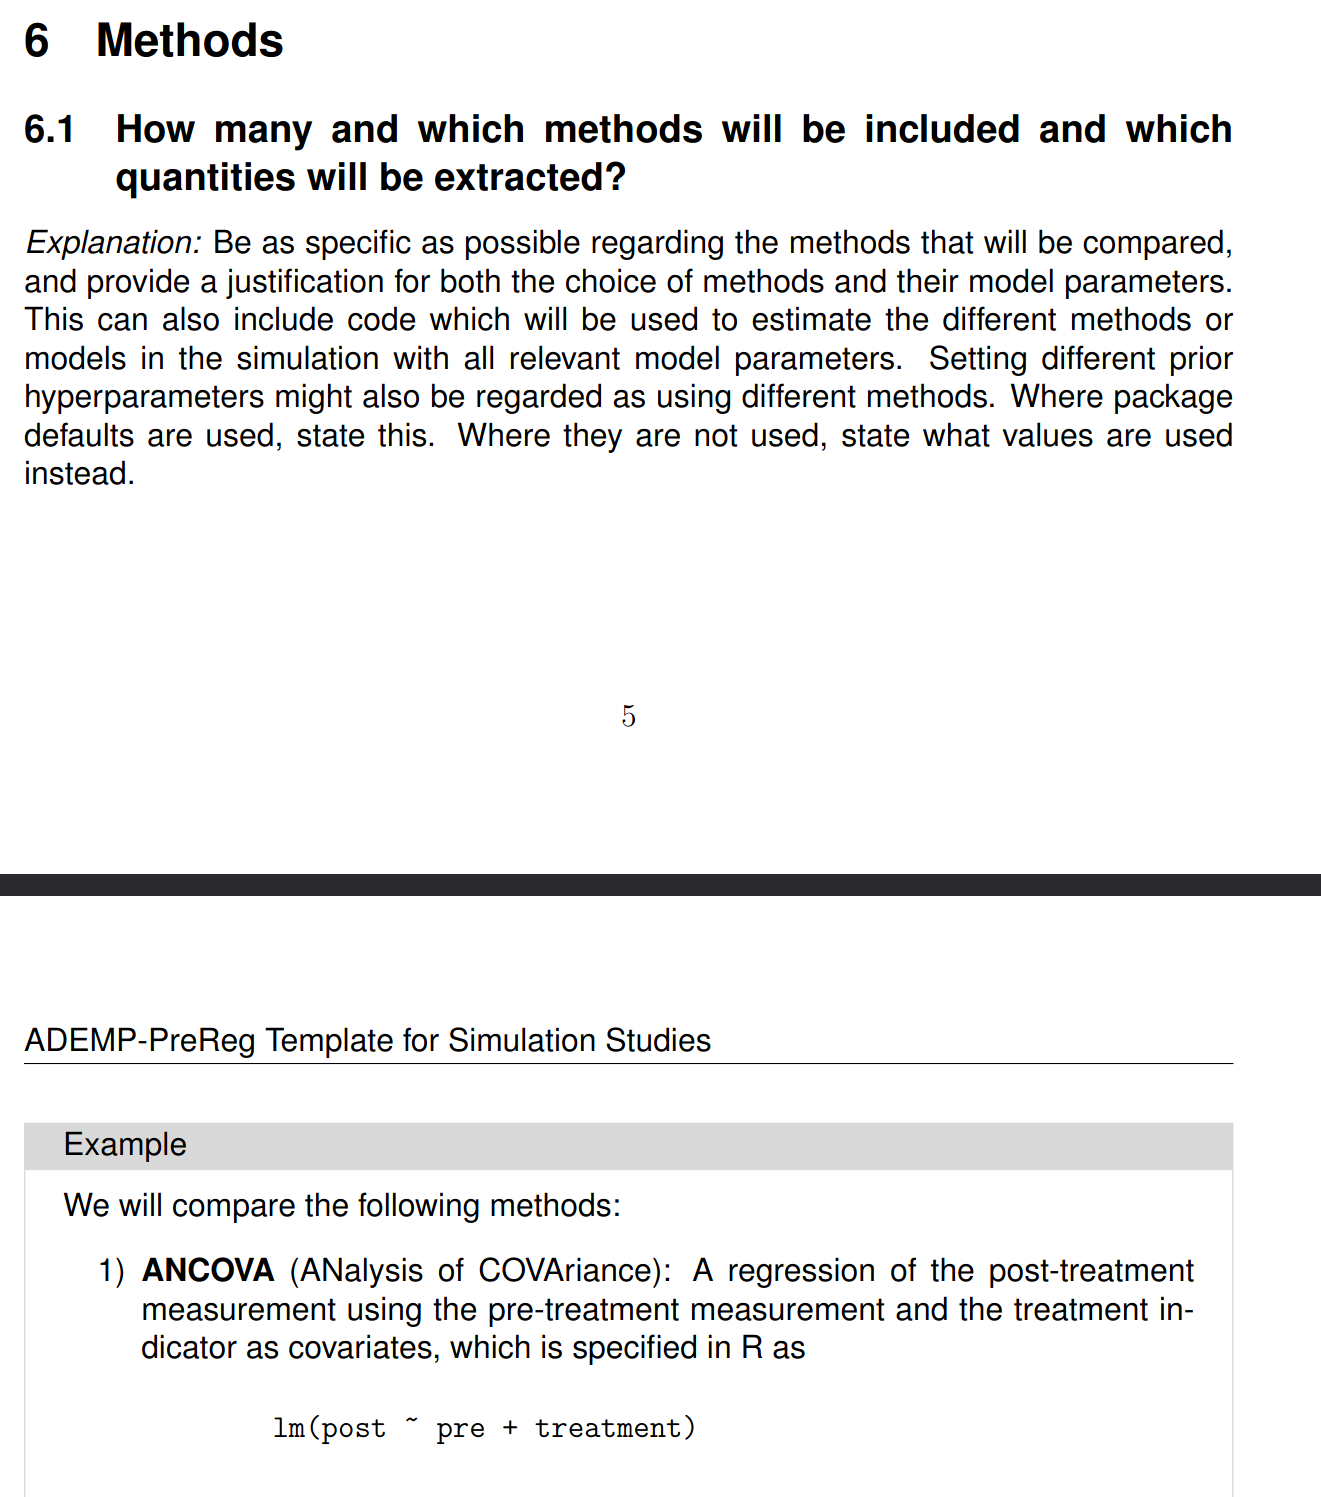
\includegraphics[width=\textwidth,frame]{pics/6methods.png}}
%     % \only<7>{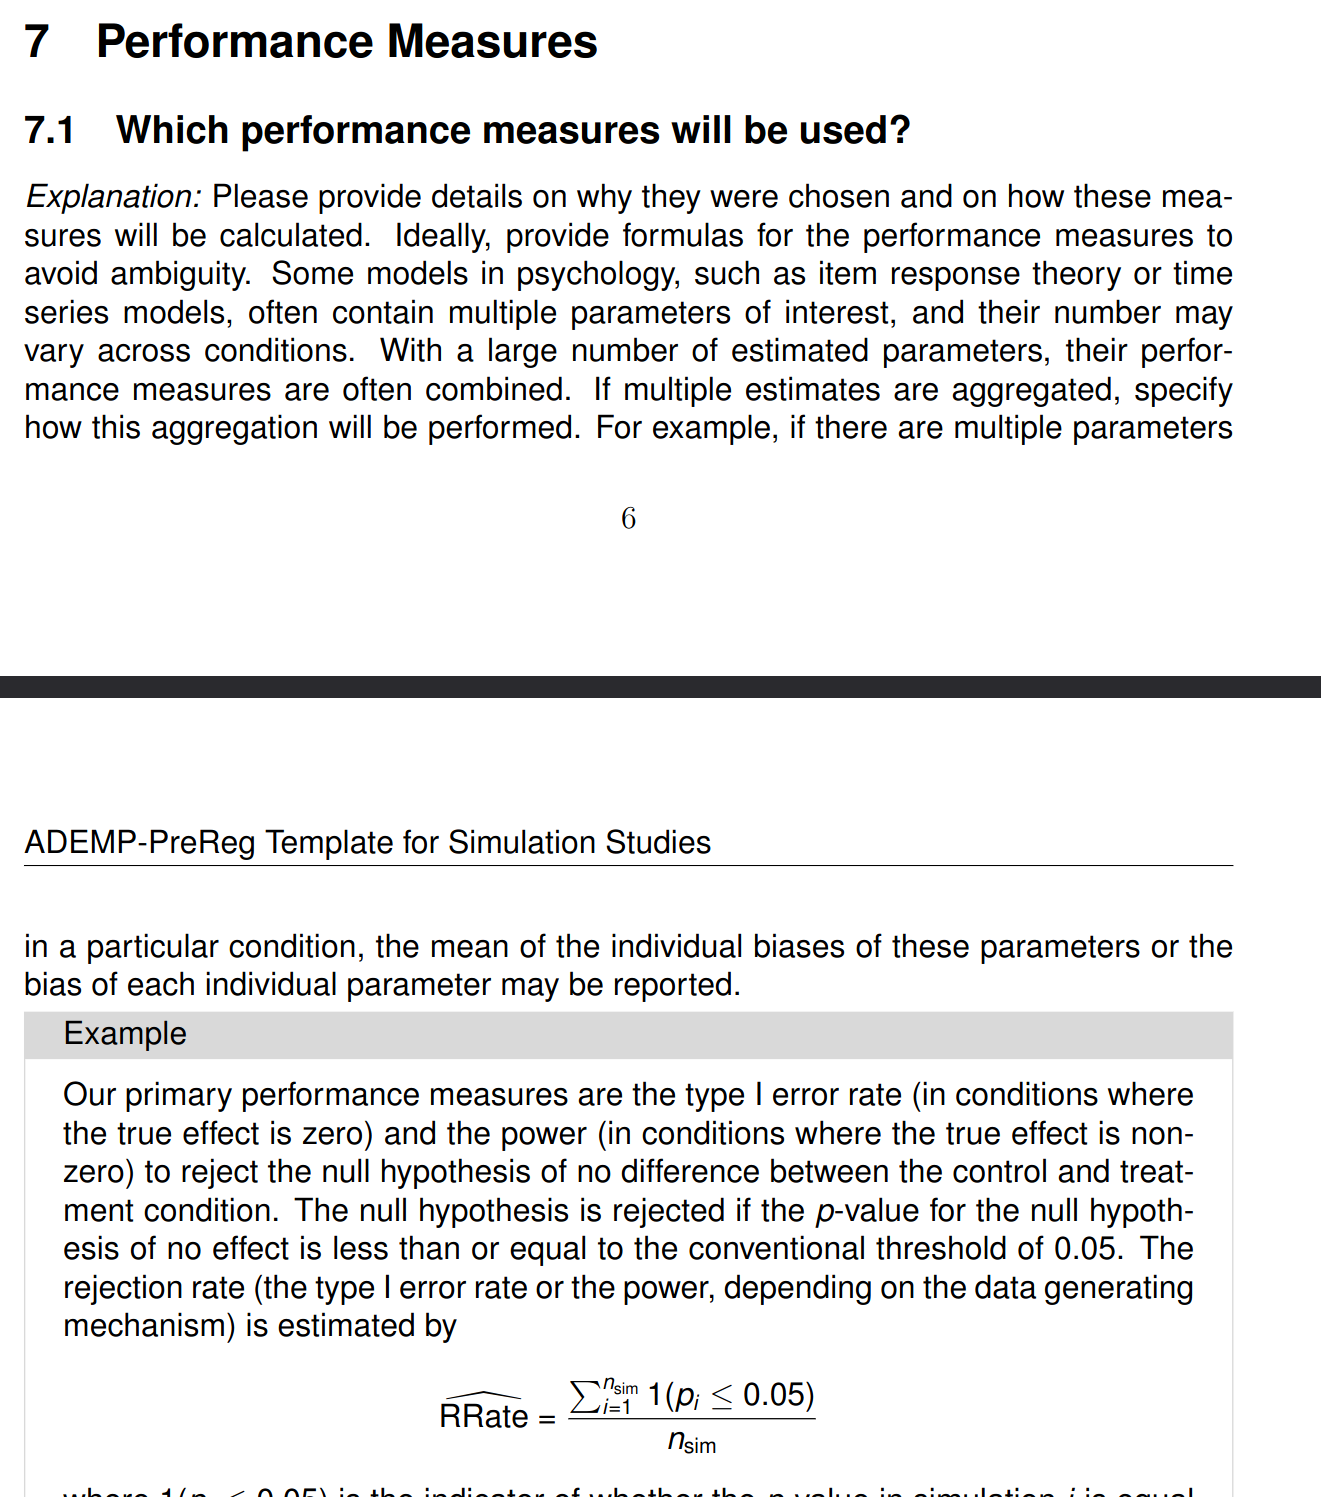
\includegraphics[width=\textwidth,frame]{pics/7performance.png}}
%     % \only<8>{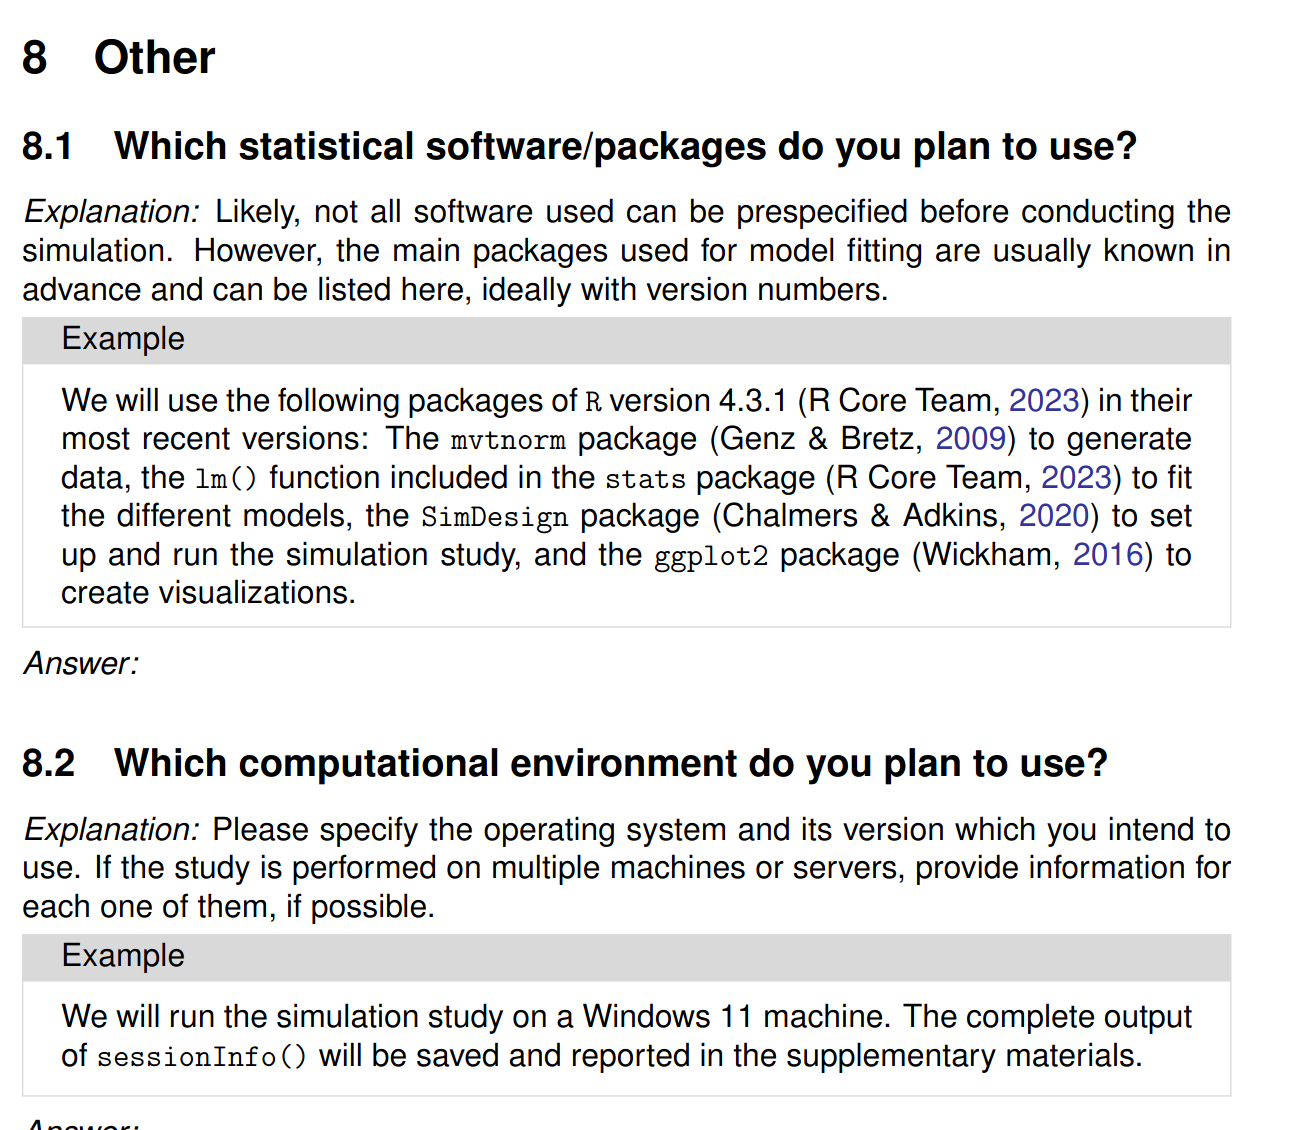
\includegraphics[width=\textwidth,frame]{pics/8other.png}}
% 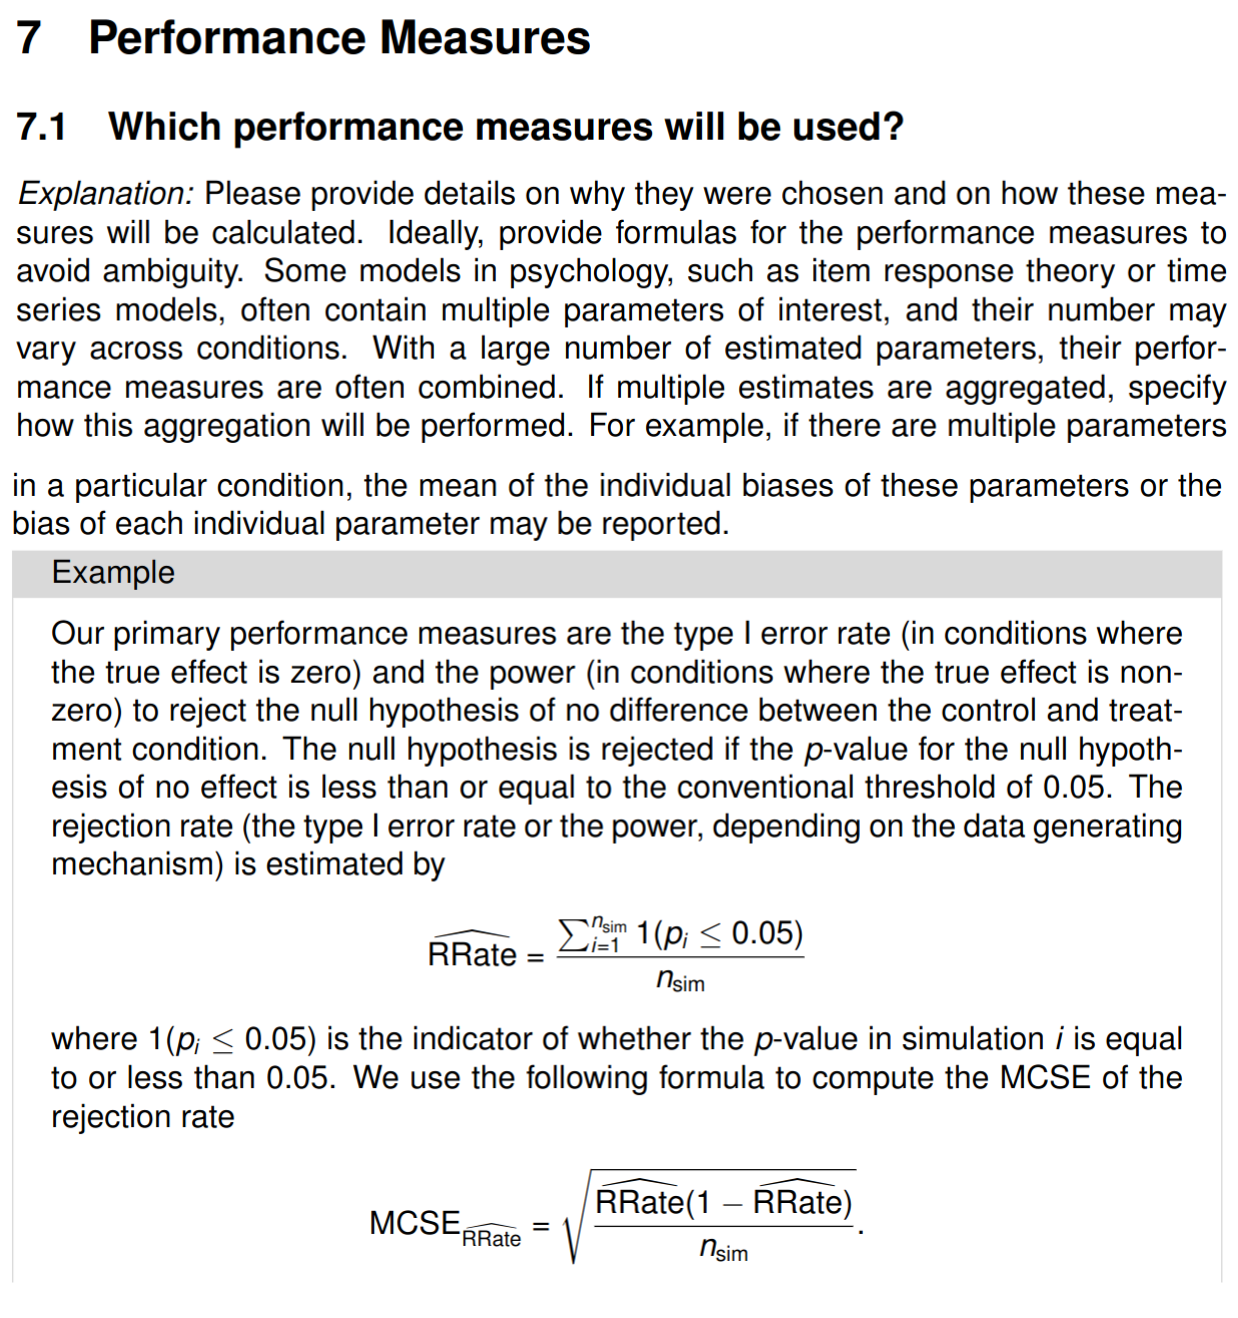
\includegraphics[width=0.9\textwidth,frame]{pics/7performance2.png}
% \end{column}
% \end{columns}
% \end{frame}

\begin{frame}{The ADEMP-PreReg template}
  \begin{columns}
    \begin{column}{0.6\textwidth}

  \begin{block}{Purposes}
    \begin{itemize}
      \pause
      \item \alert{\textbf{Planning}} of simulation studies
      \pause
      \item \alert{\textbf{Preregistration}}
      \pause
      \item Blueprint for \alert{\textbf{reporting}}
      \pause
      \item \alert{\textbf{Reviewing}} of simulation studies
    \end{itemize}
  \end{block}

  \begin{block}{Limitations}
    \begin{itemize}
    \pause
      \item Preregistration could be \alert{\textbf{faked}}
    \pause
      \item May \alert{\textbf{slow down}} exploratory research
    \end{itemize}

  \end{block}
  \end{column}
  \begin{column}{0.4\textwidth}
\centering
    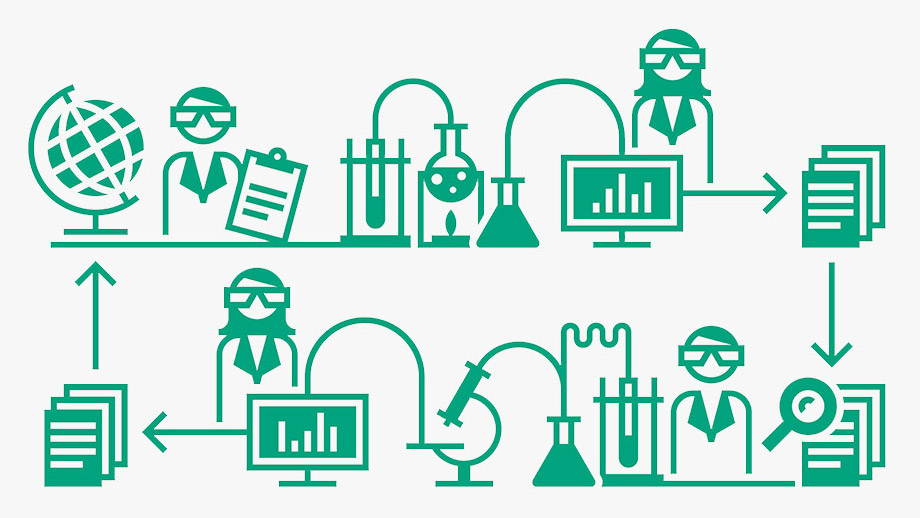
\includegraphics[width=\textwidth]{pics/CRScycle.JPG} \\
    {\tiny \color{gray} \href{https://zenodo.org/doi/10.5281/zenodo.7994221}{doi:10.5281/zenodo.7994221}}


  \end{column}
\end{columns}
\end{frame}


\begin{frame}{Conclusions}

  \begin{block}{}
    \centering
    
\includegraphics[width = 0.75\textwidth,frame]{pics/siepeetal.png}

    \begin{itemize}
    \pause
      \item Simulation studies can have \alert{\textbf{big impact}}, should be
            \alert{\textbf{conducted carefully}}
      \pause
      \item \alert{\textbf{Protocols}} can make simulation studies
            \alert{\textbf{more reliable}}
      \pause
      \item \alert{\textbf{ADEMP-PreReg template}} helps in preregistration,
            planning, reporting, reviewing of simulation studies
    \end{itemize}
  \end{block}

  {\tiny \color{gray} \href{https://doi.org/10.31234/osf.io/ufgy6}{doi.org/10.31234/osf.io/ufgy6}. Slides and preprint at \href{https://bsiepe.github.io}{https://bsiepe.github.io}.}
\end{frame}

\begin{frame}[allowframebreaks]{References}
\scriptsize
  \bibliographystyle{apalikedoiurl}
  \bibliography{bibliography.bib}
\end{frame}

\end{document}
